%   \begin{figure}[t]
%       \footnotesize
%       \centering
%       \begin{tikzpicture}[scale=0.4]
%           \pie[color={xLightGreen,xLightYellow,xLightBlue,xLightRed,gray!50}]{33/Name, 32/Word, 15/Phrase, 13/Random, 7/Other}
%       \end{tikzpicture}
%       % \begin{tikzpicture}[xscale = 1, 
%       %     font=\sffamily,
%       %     mystyle/.style={draw=white, very thick, text=black, font=\sffamily\bfseries},
%       %     ]
%       %     \pie[square,  
%       %     style={mystyle},
%       %     color={yellow!80!orange, gray, blue!40, orange}, 
%       %     text=inside,
%       %     %text=legend, 
%       %     ]{33/Name, 32/Word, 15/Phrase, 13/Random, 4/Location, 2/Org, 1}
%       % \end {tikzpicture}
%       \caption{Composition of \textbf{tags} (\hmail dataset) as a percentage. The core constituents of majority of passwords are words, names, or phrases--this supports our thesis in this paper. The total number of passwords is 7\,235, and \textit{other} is composed of 4\%: location, 2\%: organisation, and 1\%: date.}
%       \label{fig:tag-piechart}
%       \vspace{-1em}
%   \end{figure}

\section{Analysis of the Labelled Dataset}
\label{sec::chp4::results}

\begin{table}[t]
\centering
%\footnotesize
\caption{Table showing a small subset of the labelled \hmail dataset. We decomposed the passwords from the \hmail dataset into chunks, words, structure, tags, and transformations (if applicable). Such decomposition allows for better password modelling and nuanced understanding of human behaviour when creating their chosen passwords.}
\label{table:results-snippet}
    \setlength\tabcolsep{6pt} % default value: 6pt
    %\setlength{\fboxsep}{1pt} % Remove padding
    %{\renewcommand{\arraystretch}{0.3}% for the vertical padding
\begin{tabular}{llllll}
\toprule
\textbf{pwd} & \textbf{chunks} & \textbf{words} & \textbf{structure} & \textbf{tags} & \textbf{transform} \\
\midrule
estatica4 & \colorbox[HTML]{A1EEBD}{estatica}\colorbox[HTML]{F6F7C4}{4} & estatica & wd & word & \\
manterola84 & \colorbox[HTML]{A1EEBD}{manterola}\colorbox[HTML]{F6F7C4}{84} & manterola & ndd & name & \\
% onstantinopla84 & \colorbox[HTML]{A1EEBD}{onstantinopla}\colorbox[HTML]{F6F7C4}{84} & constantinopla & wdd & location & onstantinopla constantinopla \\
elingeniero20 & \colorbox[HTML]{A1EEBD}{el}\colorbox[HTML]{F6F7C4}{ingeniero}\colorbox[HTML]{F6D6D6}{20} & el ingeniero & wwdd & word & \\
centella2 & \colorbox[HTML]{A1EEBD}{centella}\colorbox[HTML]{F6F7C4}{2} & centella & wd & word & \\
indiferencia8 & \colorbox[HTML]{A1EEBD}{indiferencia}\colorbox[HTML]{F6F7C4}{8} & indiferencia & wd & word & \\
veinti7 & \colorbox[HTML]{A1EEBD}{veinti}\colorbox[HTML]{F6F7C4}{7} & veinti & wd & word & \\
tere50 & \colorbox[HTML]{A1EEBD}{tere}\colorbox[HTML]{F6F7C4}{50} & tere & wdd & word & \\
Bertita1 & \colorbox[HTML]{A1EEBD}{Bertita}\colorbox[HTML]{F6F7C4}{1} & bertita & nd & name & \\
alohanene2 & \colorbox[HTML]{A1EEBD}{aloha}\colorbox[HTML]{F6F7C4}{nene}\colorbox[HTML]{F6D6D6}{2} & aloha nene & nnd & name & \\
andreateamo3 & \colorbox[HTML]{A1EEBD}{andrea}\colorbox[HTML]{F6F7C4}{te}\colorbox[HTML]{F6D6D6}{amo}\colorbox[HTML]{7BD3EA}{3} & andrea te amo & nwwd & phrase & \\
happyness & \colorbox[HTML]{A1EEBD}{happyness} & happiness & w & word & happiness \\
\bottomrule
\end{tabular}
%} %% vertical padding
\end{table}

 This section presents an overview of some analysis of the labelled \hmail dataset. The dataset has many potential use-cases (as discussed in Section~\ref{sec::passwordninja::impact}) First, we draw some insights from this manually labelled dataset.
 
 We manually decomposed and labelled the entire \hmail dataset, comprising 8\,929 records. Specifically, we labelled 7\,235 records that were not solely numeric. Additionally, we labelled 2\,000 records from the \phpbb dataset for comparative analysis and further experiments (discussed in subsequent sections). \hyperref[table:results-snippet]{Table \ref{table:results-snippet}} provides a snapshot of the labelled dataset. Given that we labelled the dataset into \textit{chunks}, \textit{words}, \textit{structure}, \textit{tags} and \textit{transformations}, we will analyse each of these components separately in this section. This section will primary focus on the \hmail dataset as it is completely labelled and therefore can be used to draw more useful insights.

The time it takes to label a password varies due to their complexity, but we estimate c.170 hours were spent labelling the \hmail and a portion of the \phpbb dataset. A single labeller would likely need 35 to 45 days for such a task. In a subsequent experiment, two freelancers took about 5 days each to label 2\,000 records.

%\subsection{Words}
%\label{section:results:words}

%\begin{figure}[ht]
%    \centering
%    \begin{subfigure}[b]{0.45\linewidth}
%        \centering
%        \scalebox{1}{\input{figs/why_passwords/word_freq_loglog}}
%        \caption{Unique Words}
%        \label{fig:word_freq_loglog}
%    \end{subfigure}
%    \hspace{0.5cm} % Space between the two figures
%    \begin{subfigure}[b]{0.45\linewidth}
%        \centering
%        \scalebox{1}{\input{figs/why_passwords/structure_loglog}}
%        \caption{Structures}
%        \label{fig:structure_loglog}
%    \end{subfigure}
%    \caption{Charts showing the log-log plot of word and structure against their respective rank for the \hmail dataset. Words are from extracted unique passwords. The distribution of both words and structure exhibit a power law similar to Zipf's law.}
%    \label{fig:log-log-charts}
%    %\vspace{-1.5em} % Adjust the negative value to reduce the gap
%\end{figure}

\textbf{\textsc{Words.}}\: Here, words refers to a column in our dataset and it contains extracted (meaningful) information from the sliced passwords, such as words, names, locations, organisation names, and etc. If a word is transformed in the original password string then we would transform it back to the standard form, e.g. \password{g8ors} $\rightarrow$ \textit{gators}. We observed 5\,749 unique words. The frequency of the words in the unique password strings exhibit a power-law like distribution, specifically the Zipf's law. Figure \ref{fig:word_freq_loglog} shows that the log-log plot of word frequency and rank is linear: the frequency of the $n^{th}$ ranked word $f_n \propto n^{-\alpha}$ \cite{Kobayashi_Mark_Turin_2011}. This builds on the hypothesis that raw passwords (not unique) in a given dataset also exhibit the Zipf's law \cite{wang_zipfs_2017}. This has implications for how we model passwords.

%   \begin{figure}[ht]
%       \centering
%       \scalebox{0.5}{\input{figs/word_freq_loglog.tex}}
%       \caption{Plot of Rank v.s. Word Frequency (log-log scale) for the \hmail dataset. Words are extracted from the unique password strings in the dataset. The distribution exhibit a \textit{power law} similar to Zipf's law.}
%       \label{fig:word_freq_loglog}
%   \end{figure}


%   \subsection{Structures}
%   \label{section:results:structures}

\textbf{\textsc{Structure.}}\: Structure of the password indicates the order and position of different types of characters, digits and words. Table~\ref{table:structures} shows the most common structures for the \hmail dataset. Majority of the passwords are composed of words or combination of words (phrases). The most common structure is a $w$ (word), which is prone to simple dictionary attacks. 

Our method of labelling the structures is certainly up for debate, however, they are flexible and can be converted. For example, for the password \password{mialiasesANGELO1} has the structure of \texttt{wwnd}. This structure can be converted to one presented in the \pcfg model where the authors use $L_n, D_n \text{ and } S_n$ to represent alpha, digit and special variables ($n$ represents the count of the specific variable). We can extend these to include $W_n \text{ and } N_n$  for \textbf{word} and \textbf{name} variables. So, for example, password (structure: \texttt{wwndd}) can be represented as $W_2 N_1 D_1$. So, one may be able to carry out a \pcfg style attack with the knowledge of these structures.

The distribution of the structures exhibit a power law--similar to Zipf's law if we plot the frequency of the structures against their sorted Rank (as shown in Figure~\ref{fig:structure_loglog}). This can support our thesis that the core of the password is a word or a set of words (a phrase). A question for future work is whether other datasets follow a similar power law as seen in the \hmail dataset.

%   \begin{figure}[ht]
%       \centering
%       \scalebox{0.5}{\input{figs/structure_loglog.tex}}
%       \caption{Plot of Rank v.s. Structure Frequency (log-log scale) for the \hmail dataset. The distribution exhibits a \textit{power law} similar to Zipf's law.}
%       \label{fig:structure_loglog}
%   \end{figure}

%   \subsection{Tags}
%   \label{section:results:tags}

% \textbf{\textsc{Tags.}}\: The tagging of passwords in our study enables a refined analysis of their principal components, identifying whether they consist of names, words, locations, etc. This categorisation facilitates the tailoring of attack dictionaries to specific password compositions. Future research could explore if these compositional trends are consistent across other datasets.

\textbf{\textsc{Tags.}}\: Our analysis reveals that most passwords are made up of words and names. 33\% of the total 7\,235 passwords were names, 32\% words, 15\% phrases, 13\% random, 4\% location, 2\% organisation names, and 1\% dates. These are followed by phrases and passwords classified as Random, which we further divided into R1, R2, and R3 categories. Among the 7\,235 records analysed, 946 were labelled as R2, indicating a substantial proportion of passwords appear random but are vulnerable to brute-force attacks. The distribution of the remaining random passwords is as follows: 23 classified as R3 and only one as R1. Additionally, 35 passwords were identified as keyboard patterns.

% \begin{figure}[h]
%     \centering
%     \includegraphics[scale=0.6]{hotmail_structure_freq.png}
%     \caption{Caption}
%     \label{fig:hotmail-structures}
% \end{figure}

%   \subsection{Transformations}
%   \label{section:results:transformations}

\textbf{\textsc{Transformations.}}\: We observed 324 transformations in the \hmail dataset. Though the partial labelling of the \phpbb dataset revealed more intriguing word transformations. Identifying the exact nature of a transformation can be challenging, especially for non-native speakers of the language used in the passwords, leading to less than 100\% confidence in our identifications. Transformations with nearly zero confidence were labelled as \textit{R2}.

Contextual information can also reveal more information about the transformation, for example: the string \password{01well} can simply be \textit{zero}, \textit{one} and the word \textit{well}, but if we add \password{9801well} or \password{198401well} then it becomes apparent that it is \textit{orwell} (referencing the book \textit{Nineteen Eighty-Four} \cite{Orwell_Fromm_2000} by George Orwell). This example is a clear illustration of why word search and algorithmic means of labelling passwords are difficult. Such nuanced patterns make labelling difficult for a human who cannot make the connection between \textit{84} and \textit{01well} or simply doesn't have the knowledge of that specific book and author. Though the transformation is complex to the human, it still has a $d^4w$ structure. This means that it has a predictable structure that can be guessed using a mask attack.

\newpage
Transformations can also encompass multiple words, such as mingling them or altering their order. Such transformations are less frequent than those at the word level. Hence, we categorise these as \textit{phrase-level} transformations. Examples of transformations are as follows.

\noindent\begin{tikzpicture}
\node[draw,rectangle,rounded corners=2pt,inner sep=7pt,outer sep=0pt] (box) {
\begin{minipage}{\columnwidth - 20pt}
\footnotesize
\paragraph{Phrase level transformations}
\begin{itemize}[itemsep=0pt, parsep=0pt, leftmargin=10pt]
  \item \textbf{Hybridisation:}
    \begin{itemize}[itemsep=0pt, parsep=0pt, leftmargin=10pt]
        \item \textbf{Overlapping letters}: Such as \texttt{r3al0v3} $\rightarrow$ \texttt{real love}, where numbers are used to represent letters that look similar, overlapping in meaning.
        \item \textbf{Other} More complex mixing examples: \texttt{castilleo} $\rightarrow$ \texttt{leo castillo}: A rearrangement of the letters to form the correct name.
    \end{itemize}
  \item \textbf{Change of order.} Changing the order of the words or chunks in the password. \texttt{pedro te amo} $\rightarrow$ \texttt{te amo pedro}.
  \item \textbf{Repetition.} e.g. \texttt{memememe}
\end{itemize}
\end{minipage}
};
\end{tikzpicture}

%   \begin{enumerate}[itemsep=0pt, parsep=0pt, leftmargin=12pt]
%       \item \textbf{\textsc{Homophones}:} Define a function $h : \mathcal{W} \rightarrow \mathcal{W}'$ where $\mathcal{W}$ is the set of original words, and $\mathcal{W}'$ is the set of words after applying homophone substitution, such that for example, $h(\text{"2"}) = \text{"to"}$.
%   
%       \item \textbf{\textsc{1337 Speak}(1):} Define a transformation function $l_v : \mathcal{W} \rightarrow \mathcal{W}_v$ where $\mathcal{W}_v$ is the set of words after applying visual 1337 speak transformations, e.g., $l_v(\text{"9801well"}) = \text{"1984 Orwell"}$.
%       
%       \item \textbf{\textsc{1337 Speak}(2):} Similarly, define a transformation function $l_s : \mathcal{W} \rightarrow \mathcal{W}_s$ for sound-based 1337 speak transformations, e.g., $l_s(\text{"articul8"}) = \text{"articulate"}$.
%       
%       \item \textbf{\textsc{Slang}:} Define a function $s : \mathcal{W} \rightarrow \mathcal{S}$ where $\mathcal{S}$ is the set of words transformed into slang, e.g., $s(\text{"gurlz"}) = \text{"girls"}$.
%       
%       \item \textbf{\textsc{Abbreviation/Elision}:} Define a function $a : \mathcal{W} \rightarrow \mathcal{A}$ where $\mathcal{A}$ represents words after abbreviation or elision, e.g., $a(\text{"nbtwin"}) = \text{"inbetween"}$.
%       
%       \item \textbf{\textsc{Reversal}:} Define a function $r : \mathcal{W} \rightarrow \mathcal{R}$ for reversing the letters of a word, e.g., $r(\text{"drowssap"}) = \text{"password"}$.
%       
%       \item \textbf{\textsc{Syllable Swap}:} Define a function $sw : \mathcal{W} \rightarrow \mathcal{SW}$ for swapping syllables in words, e.g., $sw(\text{"wordpass"}) = \text{"password"}$.
%       
%       \item \textbf{\textsc{$+/-$ Characters}:} Define functions $p : \mathcal{W} \rightarrow \mathcal{P}^+$ and $m : \mathcal{W} \rightarrow \mathcal{P}^-$ for adding or omitting characters, e.g., $m(\text{"bloo"}) = \text{"bloom"}$.
%       
%       \item \textbf{\textsc{Elongation}:} Define a function $e : \mathcal{W} \rightarrow \mathcal{E}$ where $\mathcal{E}$ is the set of words after elongation of characters, e.g., $e(\text{"psssss"}) = \text{"ps"}$.
%       
%       \item \textbf{\textsc{Misspelling}:} Define a function $mi : \mathcal{W} \rightarrow \mathcal{MI}$ for intentional or accidental misspelling of words.
%       
%       \item \textbf{\textsc{Doubling Letters}:} Define a function $d : \mathcal{W} \rightarrow \mathcal{D}$ for doubling letters within words, e.g., $d(\text{"biiaankaa"}) = \text{"bianka"}$.
%       
%       \item \textbf{\textsc{Random $L$ or $D$ Insertion}:} Define a function $rd : \mathcal{W} \rightarrow \mathcal{RD}$ for randomly inserting letters $L$ or $D$, e.g., $rd(\text{"cancero1s"}) = \text{"cancerous"}$.
%   \end{enumerate}

\begin{figure}[ht]
\noindent\begin{tikzpicture}
\node[draw,rectangle,rounded corners=2pt,inner sep=7pt,outer sep=0pt] (box) {
\begin{minipage}{\columnwidth - 20pt}
\footnotesize
\paragraph{Word level transformations}
\begin{itemize}[itemsep=0pt, parsep=0pt, leftmargin=10pt]
  \item \textbf{Homophones.} These are words that sound similar but have different meaning, e.g. \texttt{2} $\rightarrow$ \texttt{to}
  \item \textbf{1337 speak} is the replacement of words with numbers and letters to create alternative spellings that resemble leet or 'elite' speak. This replacement would either make the word visually look or sound similar. Examples are shown in the text below.
  \begin{itemize}[itemsep=0pt, parsep=0pt, leftmargin=10pt]
    \item \textbf{Visual.} \texttt{9801well} $\rightarrow$ \texttt{1984 Orwell}: Numbers are used to resemble the visual appearance of the corresponding letters.
        \item \textbf{Sound.} \texttt{articul8} $\rightarrow$ \texttt{articulate}: The number '8' sounds like 'ate', making the word sound like 'articulate'.
        \item \textbf{Sound.} \texttt{2rus} $\rightarrow$ \texttt{trust}: The number '2' represents 'to' and the reversal of 'rus' to 'sur' makes the word 'trust'.
        \item \textbf{Sound.} \texttt{pahswrd} $\rightarrow$ \texttt{password}: Phonetic spelling that omits certain letters but still resembles the sound of 'password'.
  \end{itemize}
  \item \textbf{Slang.} Shorthand or informal language.
  \begin{itemize}[itemsep=0pt, parsep=0pt, leftmargin=10pt]
    \item \texttt{gurlz} $\rightarrow$ \texttt{girls}
    \item \texttt{luvme} $\rightarrow$ \texttt{love me}: 'luv' is a common slang for 'love'.
    \item \texttt{skure} $\rightarrow$ \texttt{secure}: Phonetic spelling of 'secure'.
  \end{itemize}
  
  \item \textbf{Elision.} Deletion of one or more sounds in the word. \texttt{nbtwin} $\rightarrow$ \texttt{inbetween}: Shorthand for 'in between'.
  \item \textbf{Abbreviation.} \texttt{atl} $\rightarrow$ \texttt{Atlanta}.
  \item \textbf{Reversal.} Flipping the letters around, as in \texttt{drowssap} $\rightarrow$ \texttt{password}.
  
  \item \textbf{Syllable swap.} Mixing up the order of syllables or parts of the word, like \texttt{wordpass} or \texttt{word\$pass}.
  
  \item \textbf{$+/-$ characters.} Omitting one or more characters from a word, such as \texttt{bloo} $\rightarrow$ \texttt{bloom} or \texttt{asasin} $\rightarrow$ \texttt{assassin}.
  
  \item \textbf{Elongation.} Extending one or more characters in a word, like \texttt{psssss} or \texttt{sammmmm}, often to convey a drawn-out pronunciation.
  
  \item \textbf{Misspelling}: Intentional or accidental incorrect spelling of words.
  
  \item \textbf{Doubling letters.} Repeating one or more letters, as in \texttt{biiaankaa} $\rightarrow$ \texttt{bianka}.
  
  \item \textbf{Random $L$ or $D$ insertion.} Inserting letters at random points, such as \texttt{cancero1s} $\rightarrow$ \texttt{cancerous} or \texttt{plu01to} $\rightarrow$ \texttt{pluto}. Often they occur between syllables in a word.
  
\end{itemize}
\end{minipage}
};
\end{tikzpicture}
\end{figure}

\begin{figure*}[bt]
    \centering
    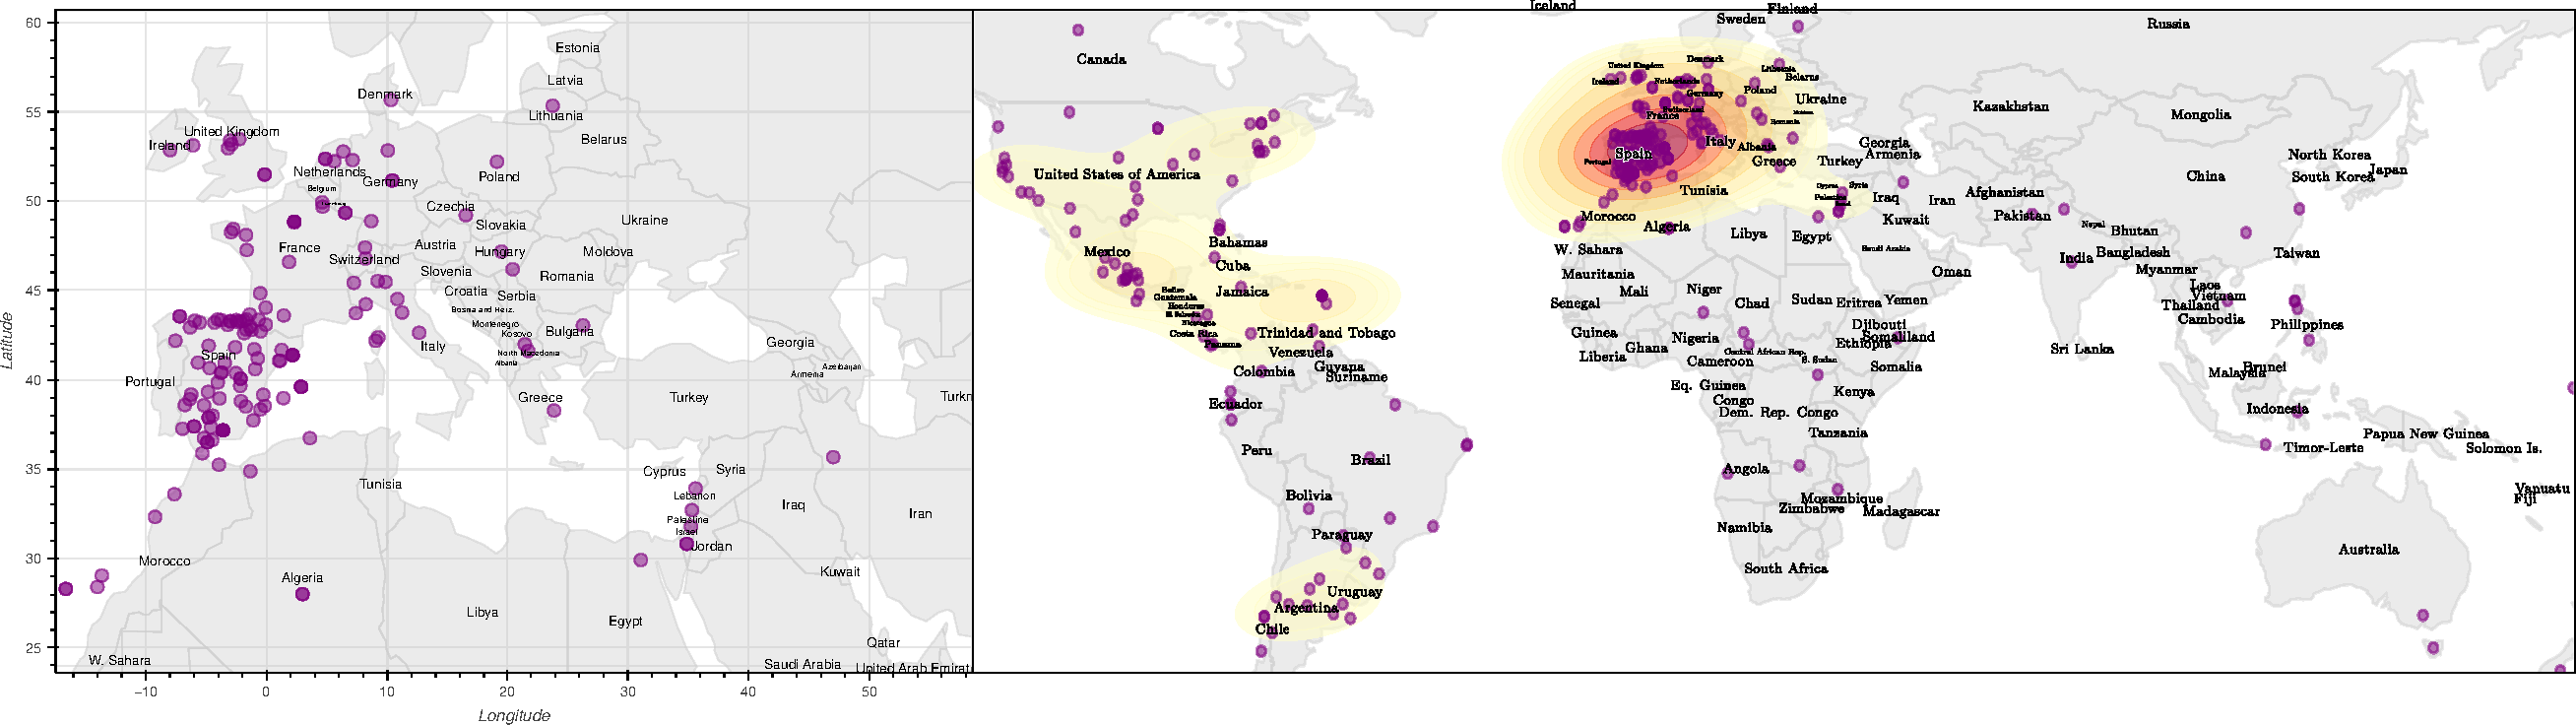
\includegraphics[scale=0.38]{figs/why_passwords/map3.pdf}
    \caption{Map showing passwords that were tagged as location in the labelled \hmail dataset. Location names were extracted from passwords, geolocated and plotted. Southern Europe, especially Spain, is more dense than other regions. This evidence and the prominent language in the \hmail dataset indicates that the passwords came from Spanish speaking regions.\\\srcOwnFig}
    \label{fig:map}
    \vspace{-1em}
\end{figure*}
\newpage
\textbf{\textsc{Location.}}\: We also embed our knowledge of geography and our surroundings into our passwords. We find that the extracted locations are correlated with the language of the users. This indicates that users are more likely to use locations that they are familiar with or are close to. Figure \ref{fig:map} shows the extracted locations on a map. Such a location-based analysis can be beneficial for post-mortem investigations in a data breach and leak. It can help identify the threat vector and the intent of the attacker.

\textbf{\textsc{Age.}}\: The age of the \hmail dataset, 2009, raises the question whether it is still relevant. One can assume that password policies and other unknown factors would have changed our behaviour and therefore the lessons-learnt from the \hmail dataset would not be significant. The machine-labelled \lizardsquad as shown in Table \ref{table:ls-structures} indicates that age of the dataset is less of a factor as we still notice similar patterns in password structures. Password composition policies however do change this pattern but not the underlying human behaviour of embedding information about ourselves and surrounding into these secrets. Moreover, we can still learn from older datasets and one can compare them to a newer labelled datasets in future studies.

